\documentclass{pnastwo}
\usepackage{color}
\usepackage{graphicx}
\usepackage{amssymb,amsfonts,amsmath}
\usepackage{lineno}
\usepackage{multirow}
\usepackage{color}
	 \definecolor{darkred}{rgb}{0.75,0,0}
	 \definecolor{darkgreen}{rgb}{0,0.5,0}
	 \definecolor{darkblue}{rgb}{0,0,0.75}
\newcommand{\cha}[1]{\textcolor{darkblue}{#1}}
\newcommand{\marcus}[1]{\textcolor{darkgreen}{#1}}


\usepackage[sort&compress]{}


\begin{document}

\title{Population dynamics of mutualisms}

 \author{
Chaitanya S. Gokhale\affil{1}{New Zealand Institute for Advanced Study, Massey University, Auckland, New Zealand} 
Marcus Frean\affil{2}{\cha{Victoria University...address details}}
}


\maketitle

\begin{article}

\begin{abstract}
Mutualistic relationships pose a conundrum for evolutionary theory.
Species that exploit other species would do better than sustaining a long drawn out mutually costly relationship. However we do see mutualistic relationships amongst even the most unlikely partners \ldots.
Eco-evolutionary dynamics \ldots
\end{abstract}


\keywords{mutualism | evolutionary game theory | multiple players
}

\tableofcontents

\cha{ToC: Just for us while we write to keep the big picture in mind}

\section{Introduction}

As with many concepts, we can trace back the study of mutualism to Aristotle \cite{aristotle:350bc}.
However formally in $1873$ the Belgian zoologist Pierre van Beneden coined the term mutualism \cite{bronstein:book:2003}.
Mutualistic relationships, interspecific interactions that benefit both species, have been empirically studied for many years 
\cite{boucher:book:1985,hinton:PTENHS:1951,wilson:AmNat:1983,bronstein:QRB:1994,pierce:ARE:2002,kiers:Nature:2003,bshary:ASB:2004} and a considerable body of theory has been put forth explaining the evolution and maintenance of such relationships \cite{poulin:JTB:1995,doebeli:PNAS:1998,noe:book:2001,johnstone:ECL:2002,bergstrom:PNAS:2003,hoeksema:AmNat:2003,akcay:PRSB:2007,bshary:Nature:2008}.
Most examples of mutualisms, including the one described by Aristotle, lend themselves to the idea of direct reciprocity \cite{trivers:QRB:1971} and have thus been extensively studied using evolutionary game theory.
The interactions in these models are usually dyadic: the fundamental interaction is between two individuals, one from each species, and the sum of many such interactions determines the evolutionary dynamics. % within each of the two species.
However, in many cases interactions between species cannot be reduced to such dyadic encounters \cite{stadler:book:2008}.

For example, in the interaction between ants and aphids or butterfly larvae \cite{pierce:BES:1987,hoelldobler:book:1990} many ants tend to each of the soft bodied creatures, providing them with shelter and protection from predation and parasites, in exchange for honeydew, a rich source of food for the ants \cite{hill:OEC:1989,stadler:book:2008}.
This is not a one-to-one interaction between a larva and an ant, but rather a one-to-many interaction from the perspective of the larva.
Another well studied example of a one-to-many interaction is that of the plant-microbe mutualism wherein leguminous hosts prefer rhizobial symbionts that fix more nitrogen \cite{kiers:Nature:2003}, or where plants provide more carbon resources to the fungal strains that are providing better access to nutrients \cite{kiers:Science:2011}.
Moving from a plant host to an animal host, a well studied example is that of the mutualistic relationship between the bioluminescent bacteria \textit{Vibrio fischeri} and \textit{Euprymna scolopes}, the bobtail squid \cite{mcfallngai:PLoSB:2014}.
In this many to one interaction, numerous bacteria are hosted in the crypts of the squids light organ.
It is costly for the bacteria to produce light but they do so while being hosted in the squid.
The bacteria mature and develop within the squid however the ones which are defective in producing bioluminescence are inevitably evicted.
Thus while the variation in the phenotypes of the interacting partners has been acknowledged, the usual analysis focuses on the interaction between the two species.

Identifying and quantifying the intraspecific variation can be a daunting task \cite{behm:JE:2014}, the intraspecific interactions are usually studied in isolation and separate from the interspecies relationships. 
While the cohorts of cleaner fish together have been taken to determine the quality of a cleaning station \cite{bshary:AB:2002,bshary:book:2003}, this can also drive variation of quality of cleaning within a cleaning station as per the interactions of individual cleaner fish amongst themselves.
In this manuscript we look at the broader picture of how the evolutionary dynamics are shaped when both the inter as well as intra species dynamics are taken together.
We find that including the full range of interactions provides us with a set of rich and intricate dynamics which are not possible when one of the dimensions is ignored.
By definition mutualistic relationships are between species.
Hence it is natural to imagine that the observed relationship may be seasonal and the interactions as not a continuous feature of the evolutionary dynamics of a single species.
Hence timing is crucial for maintaining mutualistic interactions.
In a changing ecology edits in global climate change might affect the timing of when flowers mature and when their dispersers do, quite easily disrupting the delicately balanced mutualistic interactions.
Unless both the interacting species can respond in a similar fashion the mutualism would easily break down \cite{warren:GCB:2014}.
We tackle this seasonality by changing the duration of the impact of intraspecies and interspecies dynamics.
Furthermore to complete the ecological picture we study not just the evolutionary but the population dynamics of the mutualists.
Allowing for extinctions informs us at what population densities we might expect to find mutualistic interactions in nature.
We demonstrate the crucial nature of the feedback between population and evolutionary dynamics which can maintain mutualisms preventing either or both species from going extinct. 
We make use of evolutionary game theory to analyze how benefits are shared between the two mutualistic species
\cite{weibull:book:1995,hofbauer:JMB:1996,hofbauer:book:1998}.
We begin with the previously studied interspecies dynamics as the foundational framework \cite{gokhale:PRSB:2012}.
Then we increase the complexity of the system by including intraspecies dynamics, seasonality and finally population dynamics.
The rich dynamics observed provides us with novel insights about the immense dependencies of mutualisms and the fragility of such delicately balanced interactions.

\marcus{This paragraph - is it about 1-1 vs 1-many, or dyadic vs ...?  Seems like it's setting up to be a ``Dyadic isn't enough'' para. In that case fine but the next para should be making the (main) point that intra-specific interactions are perhaps an important, and hitherto ignored, determinant of evolutionary outcomes for mutualisms.  }
\cha{This was a haphazard collection of ideas. Now I have ordered them.
\begin{itemize}
	\item First - general mutualism
\item Second - why we need more than dyadic
\item Third- Why we need intra species interactions to be included and what we show in this manuscript
\end{itemize}
Third paragraph is way too long and I think can be shortened...have a look
}


\section{Model and Results}


\begin{figure}
\begin{center}
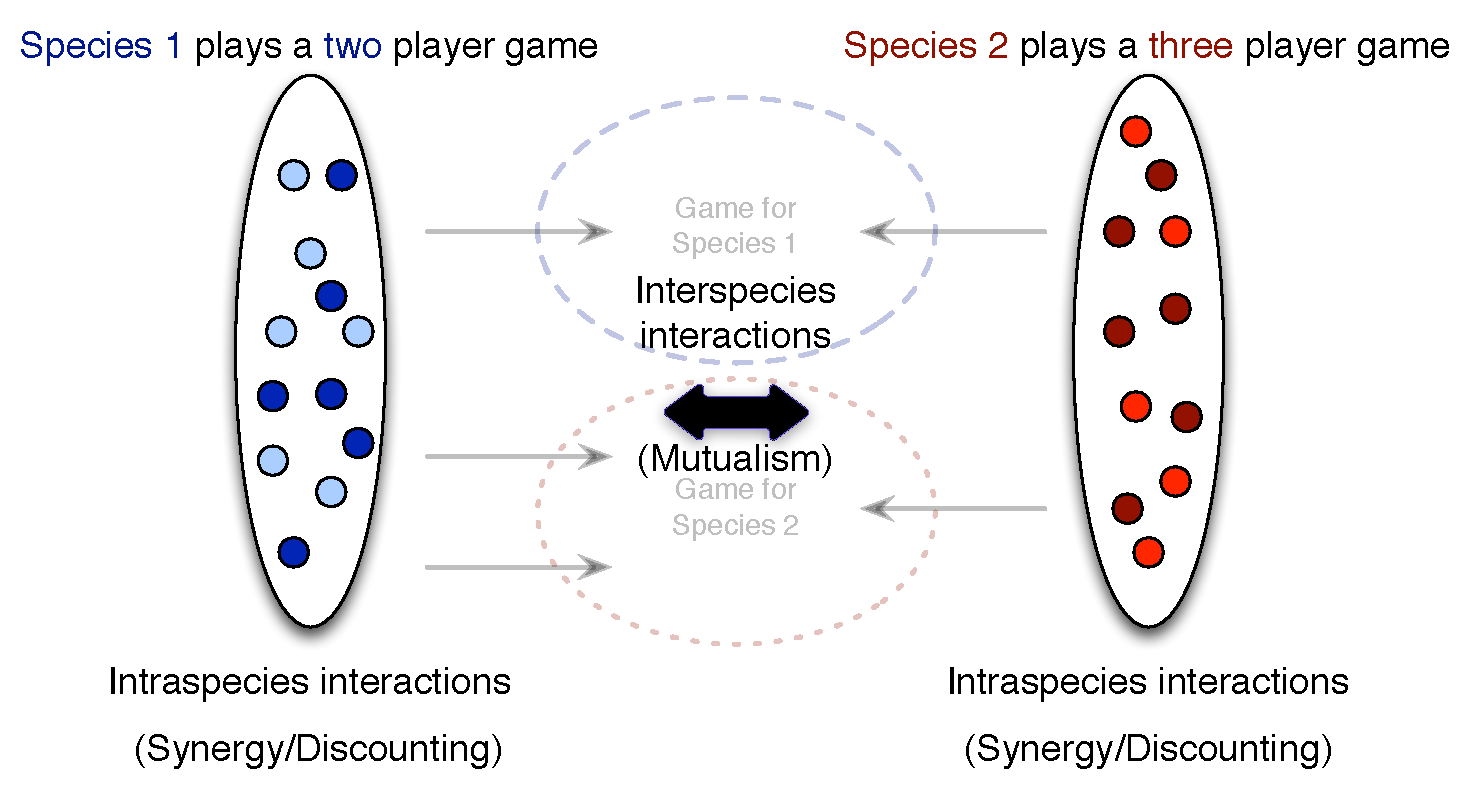
\includegraphics[width=\columnwidth]{../Figures/interintra.pdf}
\caption{
\textbf{Evolutionary dynamics with combined inter-intra species dynamics.}
We assume the interactions between species to be mutualistic described by the snowdrift game \cite{bergstrom:PNAS:2003,souza:JTB:2009,gokhale:PRSB:2012}.
Species $1$ plays a $d_1^{inter}$ player game with Species $2$ while Species $2$ plays a $d_2^{inter}$ player game.
Each species has two types of players ``Generous" and ``Selfish" who besides interacting with the members of other species, also take part in intra species dynamics.
\cha{We assume a general framework of synergy and discounting for the intraspecies interactions \cite{eshel:AmNat:1988,hauert:JTB:2006a}
}
\label{fig:conceptart}
}
\end{center}
\end{figure}



\subsection{Interspecies dynamics}

Since we focus on mutualism the interspecies dynamics is given by the multiplayer version of the snowdrift game \cite{bergstrom:PNAS:2003,souza:JTB:2009,gokhale:PRSB:2012}.
Hence both species need to contribute towards the common benefit which is generated.
However the individuals in each species could get away with contributin a bit less than other individuals.
Hence for example if producing brighter light comes at a premium for the \textit{Vibrio} in the squid then the dimmer \textit{Vibrio} would be better off (Note that not producing any light is not an option as it results in eviction).
Thus we assume that each species consists of two types of individuals ``Generous" $G$ and ``Selfish" $S$. 
Thus if everyone is ``Generous" and contributing in the generation of mutual benefits then one can get away with being a bit selfish. However both species cannot be completely ``selfish" by definition of mutualism.
This interaction framework corresponds to that of a multi player version of a snowdrift game and is discussed in detail in the Supplementary Material (SI).
Hence the pressure is on a specie in making the partner ``Generous" while getting away itself by being ``Selfish".
The fitness of each of the types within a species thus depends on the composition of the other species.
For example if the frequency of the``Generous" types in Species $1$ ($G_1$) is $x$ and that in Species $2$ ($G_2$) is $y$ then fitness of $G_1$  is given by $f^{inter}_{G_1} (y)$ and that of $G_2$ as $f^{inter}_{G_2} (x)$

\subsection{Intraspecies dynamics}

For intraspecies dynamics we do not restrict ourselves to any particular interaction structure and thus can make use of the general multiplayer evolutionary games framework \cite{gokhale:PNAS:2010,gokhale:DGAA:2014}.
Moving from the interspecies dynamics, the two types already described are ``Generous" and ``Selfish".
Thus we already have each species containing two different types of individuals.
It is possible that a different categorisation exists within a species however for the sake of simplicity we study the dynamics between ``Generous" and ``Selfish" types within a species.
However the individuals which are ``Generous" for the interspecies interaction may/may not be more giving or in a sense ``Cooperators" for intraspecies dynamics.
Thus we need a flexible cost-benefit framework to model the intraspecies dynamics which can be easily tuned to the particular situation.
The cost benefit framework described in \cite{eshel:AmNat:1988,hauert:JTB:2006a}
 allows us to transition between four classic scenarios of evolutionary dynamics \cite{nowak:Science:2004}.
For example in our case we can have a dominance of the ``Generous" type or the ``Selfish" type or both the types can invade from rare resulting in a co-existence or bistability if both pure strategies are mutually non-invasive.
For the intra species interactions the fitness of a $G_1$ is then given by $f^{intra}_{G_1} (x)$ and that of $G_2$ is given by $f^{intra}_{G_2} (y)$ and similarly for the ``Selfish" types.

\subsection{Combined dynamics}

Putting together intra and interspecific dynamics provides a complete picture of the possible interactions occurring. While we are interested in mutualism at the level of the interspecies interactions there are four possible interactions within each species \cite{nowak:Science:2004,hauert:JTB:2006a}. Since the within species interactions for the two different species do not need to be the same, there are in all sixteen different possible combinations.
Assuming additivity in the fitnesses of inter and intraspecies fitnesses, the combined fitness of each of the two types in the two species are given by,

%
\begin{align}
	f_{G_1} (x,y) &= p f^{inter}_{G_1} (y) + (1-p) f^{intra}_{G_1} (x) \nonumber \\
	f_{S_1} (x,y) &= p f^{inter}_{S_1} (y) + (1-p) f^{intra}_{S_1} (x) \nonumber \\
	f_{G_2} (x,y) &= p f^{inter}_{G_2} (x) + (1-p) f^{intra}_{G_2} (y) \\
	f_{S_2} (x,y) &= p f^{inter}_{S_2} (x) + (1-p) f^{intra}_{S_2} (y) \nonumber
\end{align}
%
The parameter $p$ tunes the impact of each of the interactions on the actual fitness that eventually drives the evolutionary dynamics.
For $p=1$ we recover the well studied case of the Red King dynamics \cite{gokhale:PRSB:2012} while for $p=0$ the dynamics of the two species are essentially decoupled and can be individually studied by the synergy/discounting framework of nonlinear social dilemmas \cite{hauert:JTB:2006a}.
Of interest in the continuum and the intermediate values of $p$.
However that would mean we need to track the qualitative dynamics of sixteen possible intraspecies dynamics as $p$ changes gradually from close to $0$ to close to $1$ (SI). 
The time evolution of the ``Generous" types in both species is then given by,

\begin{align}
\dot{x} &= r_x x \left(f_{G_1}(x,y) -  \bar{f}_1(x,y) \right) \nonumber \\
\dot{y} &= r_y y \left(f_{G_2}(x,y) -  \bar{f}_2(x,y) \right).
\label{eq:repeqs}
\end{align}


This approach provides us with a powerful method to incorporate a multitude of realistic concepts in the analysis.
For example the number of players involved in a game, which has been shown to be a crucial factor in determining the evolutionary dynamics could be different for each interactions, inter and intra species interactions for Species $1$ ($d^{inter}_1$, $d^{intra}_1$) and similarly for Species 2 ($d^{inter}_2$, $d^{intra}_2$). 
The interspecies interactions are proxied by the multiplayer Snowdrift game which can incorporate threshold effects.
For example a certain number of ``Generous" cleaner fish may be required to clean the host or a certain number of ``Generous" ants required to protect larva from predators.
We can have $M_1$ and $M_2$ as the thresholds in the two species.
Since the interaction matrices for the inter and intra species dynamics are completely different there doesn't need to be any relationship between the costs and benefits of the four games (Two snowdrift games from the perspective of each species and the intragames within each species).

We can have a diverse and rich set of dynamics possible which brings into question the study of coevolution based on only interspecies interactions. Even if we make a large number of assumptions and even if the intraspecies dynamics accounts for only $33\%$ ($1-p$) of the cumulative fitness, we can see drastically different qualitative dynamics which is capable of explaining the persistence of exploiters.

\begin{figure*}
\begin{center}
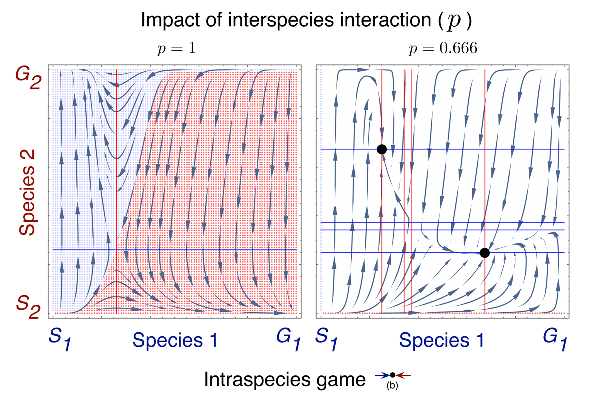
\includegraphics[width=1.5\columnwidth]{../Figures/mainexample2.pdf}
\caption{
\textbf{Change in evolutionary dynamics due to inclusion of intraspecies dynamics.} When the fitness of the ``Generous" and ``Selfish" types in both the species is solely determined by the interactions which occur between species (in this case mutualism, $p=1$) then we recover the dynamics as studied previously in \cite{gokhale:PRSB:2012}. The colours represent the initial states which result in an outcome favourable for Species $1$ (blue leading to ($S_1$,$G_2$)) and Species $2$ (red, leading to ($G_1$,$S_2$)). This can result in the red King effect and other possible complexities as discussed recently in \cite{gao:SciRep:2015}. However when we start including intraspecies dynamics the picture can be very different.
Even when the impact of intraspecies dynamics is only a $1/3$ on the total fitness of the ``Generous" and ``Selfish" types we see a very qualitatively different picture.
Two fixed points are observed where both the ``Generous" and ``Selfish" types can co-exist in both the species.
All initial states in the interior lead to either one of these fixed points (hence the lack of colours).
However it is still possible to characterize the ``successful" species as one of the equilibrium is favoured by one species than the other.
The horizontal isoclines are for Species $1$ while the vertical ones are for Species $2$.
The analysis was done for a 5 player game $d_1^{inter} = d_2^{inter} = d_1^{intra} = d_2^{intra} = 5$, $b=2$, $c=1$ and $r_x = r_y /8$ for the interspecies mutualism game while additionally $\tilde{b}_1 = \tilde{b}_2 = 10$ and $\tilde{c}_1 = \tilde{c}_2 = 1$ and $\omega_1 = \omega_2 = 3/4$ for the two intraspecies games within each species. Note that even with symmetric games within each species we can a qualitatively drastic difference when compared to the dynamics excluding intraspecies interactions.  For different intraspecies interactions within each species and for varying $p$ see SI.
\label{fig:mainexampleone}
}
\end{center}
\end{figure*}

\subsection{Population dynamics}

Until now we have considered that each species consists of two types of individuals and they make up the population of that species.
However populations sizes change over time. 
Assuming that ecological changes are fast enough that they can be averaged out, we can usually ignore their effect on the evolutionary dynamics.
It is now possible to show that evolution can happen at fast timescales, comparable to those of the ecological dynamics \cha{add citations with examples}.
Hence we need to tackle not just evolutionary but eco-evolutionary dynamics together.
%
\begin{figure}
\begin{center}
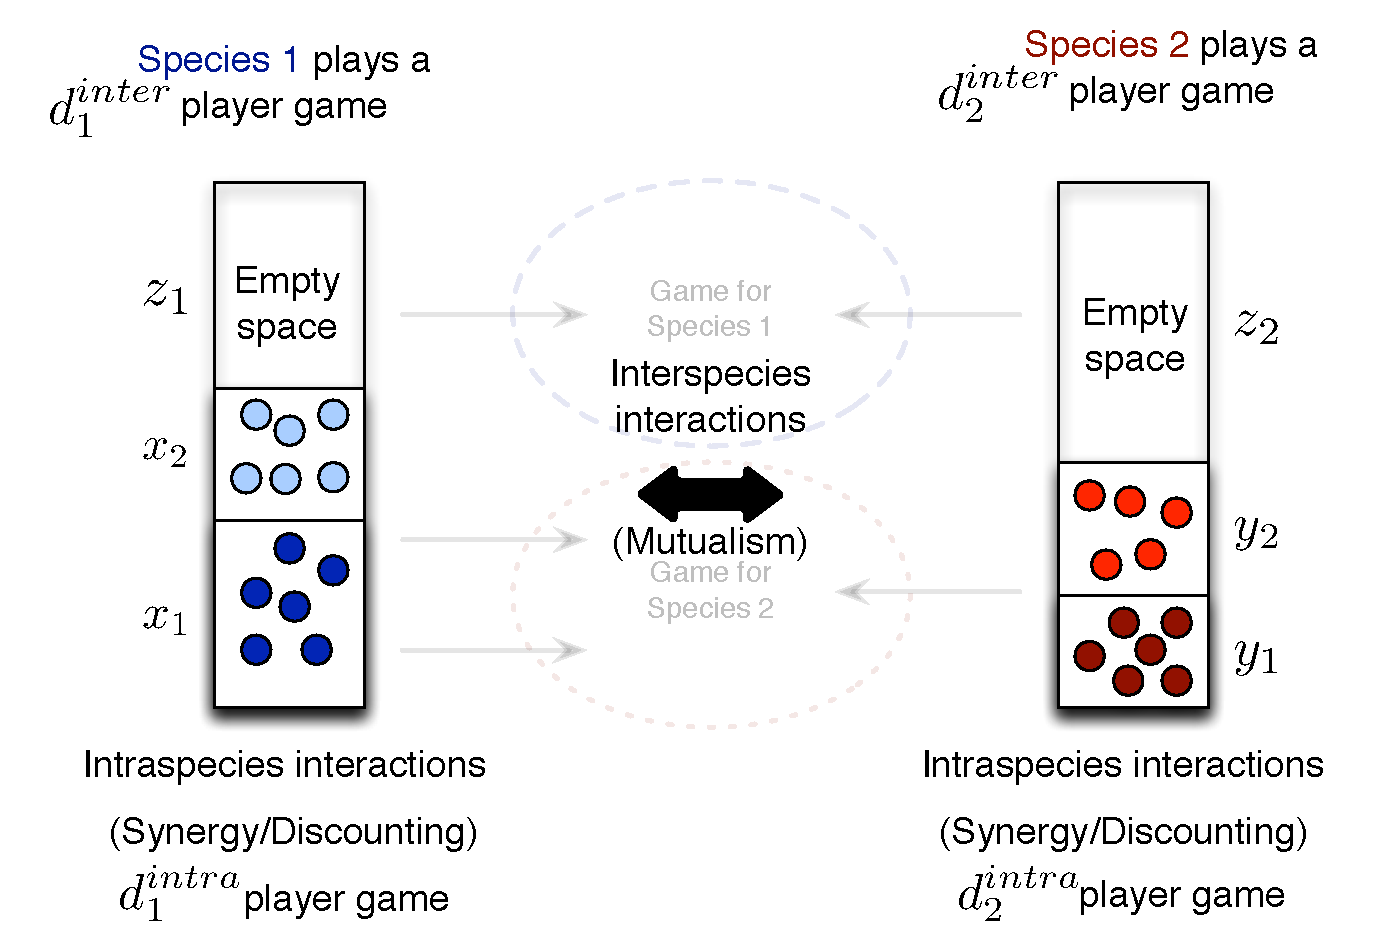
\includegraphics[width=\columnwidth]{../Figures/popdyninterintra.pdf}
\caption{
\textbf{Population and evolutionary dynamics with combined inter-intra species dynamics.}
As with the interactions described in \ref{fig:conceptart} the two species consist of two types of individuals ``Generous" and ``Selfish".
Since the two species can in principle occupy different environmental niches, they  can have non-overlapping population carrying capacities.
The normalised carrying capacity in both species is $1$ and we have $x_1 + x_2 + z_1 = 1$ (for Species $1$) where $x_1$ and $x_2$ are the densities of the ``Generous" and ``Selfish" types respectively. 
The parameter $z_1$ represents the remaining space into which the population can still expand into.
For $z_1 = 0$ the population is at its carrying capacity while for $z_1 = 0$ Species $1$ is extinct. 
\label{fig:conceptartpopdyn}
}
\end{center}
\end{figure}
%

To include population dynamics in the previously considered scenario, we reinterpret $x_1$ now as the fraction of ``Generous" types and $x_2
$ as the fraction of ``Selfish" types in Species $1$.
Also now we have $z_1 = 1 - x_1 - x_2$ as the empty spaces in the niche occupied by Species $1$. Similarly we have $y_1$, $y_2$ and $z_2$ (Fig.~\ref{fig:conceptartpopdyn}).
This approach has previously been explored in terms of social dilemmas in \cite{hauert:PRSB:2006}.
We adapt and modify it for the two species and hence now the dynamics of this complete system is determined by the following set of differential equations,
%
\begin{align}
	\dot{x_1} &= r_x x_1 (z_1 f_{G_1} - e_1) \nonumber \\
	\dot{x_2} &= r_x x_2 (z_1 f_{S_1} - e_1) \\
	\dot{z_1} &= - \dot{x_1} - \dot{x_2} \nonumber
\end{align}
%
and for species 2
\begin{align}
	\dot{y_1} &= r_y y_1 (z_2 f_{G_2} - e_2) \nonumber \\
	\dot{y_2} &= r_y y_2 (z_2 f_{S_2} - e_2) \\
	\dot{z_2} &= - \dot{y_1} - \dot{y_2} \nonumber
\end{align}
%
where we have introduced $e_1$ and $e_2$ as the death rates of the two species.
Setting $e_1 = \frac{z_1 (x_1 f_{x_1} + x_2 f_{x_2}) }{x_1 + x_2}$ and $e_2 = \frac{z_2 (y_1 f_{G_2} + y_2 f_{S_2}) }{y_1 + y_2}$ we recover the two species replicator dynamics as in Eqs.~\ref{eq:repeqs} (For the sake of brevity we avoid showing the fitnesses in their the functional forms).
In this setup however the fitnesses need to be re-evaluated as not we need to account for the presence of empty spaces (See SI).
The dynamics is simplified by focusing on the proportion of ``Generous" types in both the species thus $g_1 = x_1/(1-z_1)$ and $g_2 = y_1/(1-z_2)$ whose time evolution is given by,
\begin{align}
	\dot{g_1} &= r_x z_1 g_1 (1-g_1) (f_{G_1} - f_{S_1}) \nonumber \\
	\dot{z_1} &= e_1 (1-z_1) - r_x z_1 (1-z_1) (g_1 f_{G_1} -  (1-g_1) f_{S_1})
\end{align}
and
\begin{align}
	\dot{g_2} &= r_y z_2 g_2 (1-g_2) (f_{G_2} - f_{S_2}) \nonumber \\
	\dot{z_2} &= e_2 (1-z_2) - r_y z_2 (1-z_2) (g_2 f_{G_2} -  (1-g_2) f_{S_2})
\end{align}
%
where everywhere we have $x_1 = g_1 (1-z_1)$ (with $x_2 = (1-g_1) (1-z_1)$) and $y_1 = g_2 (1-z_2)$ (with $y_2 = (1-g_2) (1-z_2)$) in the fitnesses as well.

Such a two species multi-type interaction system is a complicated as well as a realistic depiction of most of the mutualisms observed in nature.
However even with this complexity, the reduction of variables from six to four allows us to study the eco-evolutionary dynamics of the mutualism by looking at the two species simultaneously.
As shown in Figure \ref{fig:popdyn} we plot the evolutionary information (fraction of ``Generous" in each species) against the ecological parameter, the population density (or rather in this case the empty space which is $1-z_{1/2}$ population density).

\begin{figure*}
\begin{center}
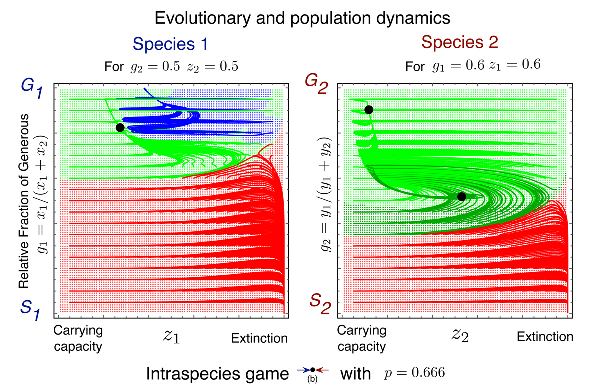
\includegraphics[width=1.6\columnwidth]{../Figures/mainexamplepopdyn2.pdf}
\caption{
\cha{\textbf{Dynamics of evolutionary strategies and population density for an intraspecies coexistence game with interspecies mutualism.}
With exactly the same parameters as that of Figure \ref{fig:mainexampleone} with  symmetric death rates $e_1 = e_2 = 0.05$.
}
}
\end{center}
\end{figure*}




\section{Discussion}


\cha{Random placement of Text}

Usually when interspecies relationships such as mutualism (or antagonist relationships as in predator-prey) are considered, the within species interactions are ignored for the sake of convenience. Including intraspecies interactions can however result in qualitatively different and rich dynamics.
In fact the coevolutionary dynamics between the two species is determined together by the inter as well as the intraspecific interactions.

%Consider two species ($1/2$) occupying different niches in an ecosystem.
%Thus we assume them to have independent carrying capacities. Each species has a normalized carrying capacity of $1$. Each species has two types the \textit{``Generous"} ones ($G_{1/2}$) who invest in a mutualistic relationship with the other species and \textit{``Selfish"} ones ($S_{1/2}$) who invest much less than their counterparts. The densities of the two types are denoted by $x_{1/2}$ and $y_{1/2}$ respectively which can sum up to the carrying capacity or not thus resulting in possible empty spaces in the niche $z_{1,2}$. Thus in all we have $x_{1/2} + y_{1/2} + z_{1/2} = 1$.
%Thus how the population densities change over time $x_{1/2} + y(1/2)$ can give us a picture of the population dynamics.
%The two species are assumed to be engaged in a mutualistic relationship. This can be aptly described by a snowdrift game \cite{souza:JTB:2009}. In a general form, a number of individuals from one species interacts with a number of individuals from the other species (excluding intra species interactions) \cite{gokhale:PRSB:2012}. 
%The densities of the two types of individuals in each species \textit{``Generous"} and \textit{``Selfish"} can be interpreted as probabilities of picking the two types. Thus the evolution of the fraction of one of the types, say \textit{``Generous"} over time provides us with the relevant evolutionary dynamics. The fraction of \textit{``Generous"} players is given by $f_{1/2} = x_{1/2} / (1- z_{1/2} )$.

\begin{acknowledgments}
Thanks for all the fish
\end{acknowledgments}




\bibliographystyle{pnas}
\bibliography{\string~/Bibtex/et.bib}


\end{article}
\end{document}
